\documentclass[conference]{IEEEtran}
\IEEEoverridecommandlockouts

% Packages
\usepackage{cite}
\usepackage{amsmath,amsfonts}
\usepackage{algorithm}
\usepackage{algpseudocode}
\usepackage{graphicx}
\usepackage{textcomp}
\usepackage{xcolor}
\usepackage{booktabs}
\usepackage{adjustbox}
\usepackage{listings}

\usepackage{verbatim}
\usepackage{multirow}

\def\BibTeX{{\rm B\kern-.05em{\sc i\kern-.025em b}\kern-.08em
    T\kern-.1667em\lower.7ex\hbox{E}\kern-.125emX}}

\begin{document}

\title{Deliverable report \\
\footnotesize \textit{"Vittorio Polci": Mat: 257817, \texttt{vittorio.polci@unitn.it}, GitRepo: \texttt{https://github.com/vittorio01/GPU-Computing-2025-257817}}}

\maketitle

\begin{abstract}
This deliverable discusses about the implementation of different parallel solutions of the SpVM algorithm between CSR matrices and a general vector,
with a final benchmark that compares all solution toghether. 

\end{abstract}

\begin{IEEEkeywords}
Sparse Matrix, SpMV, CUDA, Parallelization, Storage Format
\end{IEEEkeywords}

\section{Introduction}
The algorithm of sparse matrix-dense vector multiplication (SpMV) is an optimized version of the traditional matrix-vector multiplication
designed to handle cases where the matrix is organized in a low density of non-zero entries. 
This technique is particularly useful in scenarios that involves very large sparse matrices because it allows to reduce the used space for 
storing that large structures and, at the same time, optimizes memory access patterns during computational steps. 

Because the SpMV multiplication should handle matrices with millions or billions of not null elements, to obtain good results is necessary to use parallelization techniques 
on GPUs rather than sequential solution for CPUs. 

\section{Problem Statement}
In the SpVM multiplication we consider a matrix coded in a sparse format (in this case the CSR format) and an input vector that has the same size of its columns number. 

Each elements of the resulting vector is computed by performing the dot products of each not null elements of the matrix with the input vector and accumulating them in the corresponding row position.
At this point the main objectives are:
\begin{enumerate}
    \item Create a first sequential algorithm that performs the same operation on a sparse CSR matrix.
    \item Parallelize the first CPU implementation with CUDA and compare them in terms of performances and resurces utilization. 
\end{enumerate}

\subsection{Storage Format}
The CSR for sparse matrices is a storage format that involves three different arrays to represent the information: 
\begin{itemize}
    \item The data array, that contains all not null terms of the original matrix.
    \item The column array, where for each element in the data vector specifies its column coordinate.
    \item The row array, which contains the start and the end pointers for each row to the data and column arrays. these two pair of pointers indicates which nut null terms in the data array are contained in that specific row. 
\end{itemize}
The size of the data and column arrays depends on the number of not null elements and the size of the row array depends on the number of the rows in the original matrix. 
\begin{figure}[H]
    \centering
    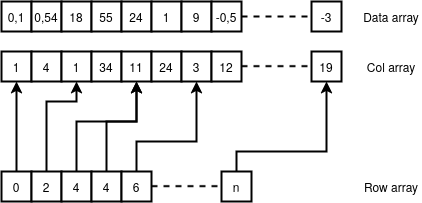
\includegraphics[width=0.8\linewidth]{images/CSR.png}
    \caption{Data organization in CSR structure}
    \label{fig:csr-format}
\end{figure}

\subsection{Parallelization}
To improve the overall performance, the parallel implementations of the first algorithm are designed to be executed on Nvidia GPUs and programmed in CUDA.
The CUDA language model permits to run a kernel on different concurrent threads called CUDA cores, where each thread represents a computational unit located in the GPU. 

In general, the workload can be splitted in different ways for a certain number of CUDA cores and different organizations can provide more or less performance in terms of the execution time and 
troughput. 

\section{State of the Art}
There already are multiple c++ libraries that performs CSR SpMV multiplications like:
\begin{itemize}
    \item cuSPARSE\cite{cuSPARSE}, the official library supported by Nvidia that can perform multiplication between matrices and vectors in different formats with CUDA. 
    \item Ginkgo\cite{ginkgo}, like MAGMA offers high-performance solution for multicore linear algebra algorithms for different platforms.
\end{itemize}
\section{Methodology and Contributions}\label{sec:methodology}
\subsection{Sequential algorithm}
The most intuitive and efficient way to perform a sequential SpMV multiplication is to scan the row vector and, using the 
stored pointers, perform the product of the corredpondent not null elements and accumulate the result in a local variable.

\begin{algorithm}[h!]
\caption{Sequential version for the SpVM algorithm}
\algorithmicrequire~Two vector structures $input$ and $output$ and a CSR matrix structure $matrix$.
\begin{algorithmic}[1]
\Procedure{vmcsrMul}{$output$, $matrix$, $input$}
\For{$i$ in $matrix.rowSize$}
\State $startRow=matrix.rowArray[i]$
\State $endRow=matrix.rowArray[i+1]$
\State $acc=0$
\For{$j$ in ${startRow,\dots,endRow}$}
\State $col=matrix.colArray[j]$
\State $acc+=$
\State $matrix.dataArray[j]*input.dataArray[col]$
\EndFor
\State $output.dataArray[i]=acc$
\EndFor
\EndProcedure
\end{algorithmic}
\label{alg:sequential}
\end{algorithm}
The algorithm \ref{alg:sequential}:
\begin{enumerate}
    \item Scans the row array and decodes each pair of start and end pointes.
    \item Using a second loop performs the product of each not null element with their correpondent elements in the input vector and accumulates the results in the variable $acc$.
    \item Stores the accumulated value in the output vector.
\end{enumerate}
The memory access pattern of this solution permits coalescent accesses in all three arrays of the sparse matrix. 
The only aspect that limits the performance of the algorithm is the access pattern for gathering the input vector elements for the multiplication
because it depends on the column coordinates stored in the column array of the matrix. 

\subsection{First parallel implementation}
A first parallel implementation of the algorithm \ref{alg:sequential} divides the workload between threads such a way that each thread processes one or more entire rows

The first operation that the algorithm performs is divide the workload for each thread. In particular:
\begin{enumerate}
    \item The row array is splitted in equal subsection that will be assigned to different blocks of threads using the ceiling division system. 
    \item The obtained subsection are then divided in the same way in order to assign equal workload to each thread.
\end{enumerate}
\begin{figure}[H]
    \centering
    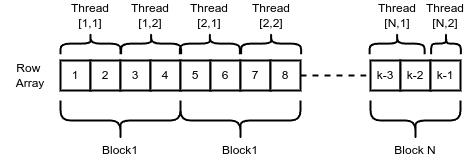
\includegraphics[width=1\linewidth]{images/ceiling_division.png}
    \caption{Example of workload division for the first parallel implementation (N blocks of 2 threads)}
    \label{fig:ceiling1}
\end{figure}
After that procedure, each thread has his number of row to process $rowsPerThread$, the start position $threadStart$ and the end position $threadEnd$ in the row array.
\begin{algorithm}[h!]
\caption{First parallelization for the SpVM algorithm}
\algorithmicrequire~Same requirements in the sequential implementation but with all structures loaded in the global memory.
\begin{algorithmic}[1]
\Procedure{vmcsrMul}{$output$, $matrix$, $input$}
\State $threadStart,threadEnd$ \Comment{Ceiling division process}
\For{$row$ in ${threadStart,\dots,threadEnd}$}
\State $startRow=matrix.rowArray[i]$
\State $endRow=matrix.rowArray[i+1]$
\State $acc=0$
\For{$j$ in ${startRow,\dots,endRow}$}
\State $col=matrix.colArray[j]$
\State $acc+=$
\State $matrix.dataArray[j]*input.dataArray[col]$
\EndFor
\State $output.dataArray[row]=acc$
\EndFor
\EndProcedure
\end{algorithmic}
\label{alg:parallel1}
\end{algorithm}

The algorithm \ref{alg:parallel1} is the simplest implementation and has good performances for common sparse matrices because:
\begin{itemize}
    \item For each thread the accesses are coalescent in all arrays of the matrix.
    \item Each thread works on the single rows independently and there is not concurrency at all. 
\end{itemize}


\subsection{Second parallel implementation}
One problem of the algorithm \ref{alg:parallel1} is that if there are threads that have much more more workload to perform respect others, the computational time 
might be affected negatively. 

This is the case for matrices which have consecutive rows that contains much more not null elements compared to the others.

A solution that may mitigate this problem is to use a dynamic assignment of the rows to threads that are in the same block:
\begin{enumerate}
    \item The row array is splitted in equal subsection for different blocks using again the ceiling division. 
    \item For each block a variable in the shared memory $pendingRow$ is initialized and used to contain the next row number that is waiting for the assignment. 
    \item Each thread uses the function $atomicAdd(pendingRow,1)$ to increment the value of $pendingRow$ and, at the same time, read its content
    \item Using the value obtained each thread computes the corresponding row and repeats step 3 and 4 until the block reach the end of its subsection. 
\end{enumerate}

\begin{algorithm}[h!]
\caption{Second parallelization for the SpVM algorithm}
\algorithmicrequire~Same requirements as the algorithm \ref{alg:parallel1}.
\begin{algorithmic}[1]
\Procedure{vmcsrMul}{$output$, $matrix$, $input$}
\State $blockStart,blockEnd$ \Comment{Ceiling division}
\State $pendingRow=0$ \Comment(only thread 0);
\State $syncthreads()$
\While {${true}$}
\State $pendingRow=atomicAdd(pendingRow,1)$
\State $+blockStart$
\If {$pendingRow>blockEnd$} \Return \EndIf
\State $startRow=matrix.rowArray[pendingRow]$
\State $endRow=matrix.rowArray[pendingRow+1]$
\State $acc=0$
\For{$j$ in ${startRow,\dots,endRow}$}
\State $col=matrix.colArray[j]$
\State $acc+=$
\State $matrix.dataArray[j]*input.dataArray[col]$
\EndFor
\State $output.dataArray[pendingRow]=acc$
\EndWhile
\EndProcedure
\end{algorithmic}
\label{alg:parallel2}
\end{algorithm}

This dynamic assignment for threads in the same block implemented in the algorithm \ref{alg:parallel2} tries to mitigate the unbalanced workload introduced in some rows. 
In facts, if some thread spend too much time when computing a single row, other available threads may perform also rows that in the algorithm \ref{alg:parallel1} should be reserved for others.  

Two possible limitation in terms of performance introduced with this system are that:
\begin{itemize}
    \item Now there is concurrency for the value $pendingRow$ that may limit the performance. 
    \item Threads may elaborate rows that are not orgainzed in a coalescent way in the data and column arrays. 
\end{itemize}

\subsection{Third parallel implementation}
Another tentative to distribute the workload contained in the single rows is to parallelize the algorithm such that each row is assigned to 
single blocks instead of threads:
\begin{enumerate}
    \item The row array is splitted for different blocks as usual. 
    \item Each block initializes at 0 their corresponding part in the output vector. 
    \item For each row all threads does some multiplication (or not) of a certain number of elements and accumulates the result in the output vector using the function $atomicAdd()$. 
\end{enumerate}

\begin{algorithm}[h!]
\caption{Second parallelization for the SpVM algorithm}
\algorithmicrequire~Same requirements as the algorithm \ref{alg:parallel1}.
\begin{algorithmic}[1]
\Procedure{vmcsrMul}{$output$, $matrix$, $input$}
\State $blockStart,blockEnd$ \Comment{Ceiling division}
\State \text{\dots}\Comment{output vector initialization phase}
\For{$row$ in ${blockStart,\dots,blockEnd}$}
\State $startRow=matrix.rowArray[row]$
\State $endRow=matrix.rowArray[row+1]$
\State $elements=endRow-startRow$
\If{$elements<blockSize.x$}
\State $col=matrix.colArray[j]$
\State $atomicAdd($
\State $output.dataArray[row],$
\State $matrix.dataArray[threadIdx.x]*$
\State $input.dataArray[col])$
\Else 
\State $threadStart,$
\State $threadEnd$ \Comment {Ceiling division on row}
\State $acc=0$
\For{$j$ in ${threadStart,\dots,threadEnd}$}
\State $col=matrix.colArray[j]$
\State $acc+=matrix.dataArray[j]*$
\State $input.dataArray[col]$
\EndFor
\State $atomicAdd($
\State $output.dataArray[row],acc)$
\EndIf
\EndFor
\EndProcedure
\end{algorithmic}
\label{alg:parallel3}
\end{algorithm}

The orgnization of algorithm \ref{alg:parallel3} distributes the workload of a row on blocks of threads instead single threads without using shared memory optimization. 

This situation may create more overhead because:
\begin{itemize}
    \item If the block size is large the function $atomicAdd()$ creates a barrier that limits too much the performance because it must guarantee atomic accumulation on the output vector. 
    \item The first threads in a block are overused for all rows but the last threads are used only if the number of rows are large enough to require them. 
\end{itemize}

\section{System Description and Experimental Set-up}
\subsection{Dataset description}
A dataset composed by 6 matrices is used for testing and benchmark all four algorithms. These matrices containes a number of not null elements between 1 and 1,5 million of not null elements and they have different organization of the elements and dispersion that challenges the algorithms in different ways:
The used dataset is obtained from the SuiteSparse Matrix Collection \cite{suitesparse}, a website that contains sample matrices which can be used for benchmarking algorithms. 

\begin{table}[h]
    \centering
    \begin{adjustbox}{width=\columnwidth}
    \begin{tabular}{llllrl}
    \toprule
    \textbf{Dataset} & \textbf{Dimension (R x C)} & \textbf{Non-zero entries} & \textbf{Type} \\
    \midrule
    dbir2 \cite{dbir2} & 18,906 x 45,887 & 1,158,159 & Unbalanced rows \\
    ex11 \cite{ex11} & 16,614 x 16,614 & 1,096,948  & Diagonally distributed (low density) \\
    language \cite{language} & 399,130 x 199,130 & 1,216,334 & Upper triangular \\
    Linux\_call\_graph \cite{linuxcallgraph} & 324,085 x 324,085 & 1,208,908 & Dense matrix (worst case) \\
    nemeth24 \cite{nemeth24} & 9,506 x 9,506 & 1,506,550 & Diagonally distributed (best case) \\
    twotone \cite{twotone} & 120,750 x 120,750 & 1,206,265 & Diagonally distributed (moderate dispersion) \\
    \bottomrule
    \end{tabular}
    \end{adjustbox}
    \vspace{1em}
    \caption{Structural patterns of the benchmark sparse matrices.}
    \label{tab:my_label}
\end{table}

\subsection{System Description}
The system used for the execution of the benchmarks is uses CUDA 12.3.2, GCC 11.5.0, and is composed by a Intel(R) Xeon(R) Silver 4214 CPU and A Nvidia A30 GPU.  

\begin{table}[h]
    \centering
    \begin{adjustbox}{width=0.8\columnwidth}
    \begin{tabular}{lll}
    \toprule
    \textbf{Characteristic} & \textbf{Value} & \textbf{Device}\\
    \midrule
    Global memory & 24 GB &  \multirow{5}{*}{\textbf{GPU: Nvidia A30}} \\
    Theoretical BW & 933 GB/s \\
    CUDA Cores & 10752 \\
    SM Number & 108 \\
    FP32 Performance & 10.3 TFLOPS \\
    \midrule 
    Cores number & 12 & \multirow{3}{*}{\textbf{CPU: Intel(R) Xeon(R) Silver 4214}} \\
    Threads number & 24 \\
    Clock speed & 2.2Ghz \\
    \bottomrule
    \end{tabular}
    \end{adjustbox}
    \vspace{1em}
    \caption{Benchmark system specs}
    \label{tab:benchmarkSystem}
\end{table}

\subsection{Experimental Set-up}
The performance is measured using the execution time elapsed measured with the C function $getTimeOfDay()$ for the sequential algorithm and $cudaEventRecord$ functions for CUDA algorithms. 

Each algorithm is executed 25 times (5 warmup cycles and 20 iterations) and from the execution times (in milliseconds) is performed the geometric mean to remove eventual outlayers. 

From the average execution time is then performed the effective bandwidth and the FLOP/s.

\begin{equation}
effBW (GB/s)=\frac{readedBytes+writtenBytes}{executionTime(ms)}*10^{-6}
\end{equation}

\begin{equation}
GFLOPS/s= \frac{2*notNull}{executionTime(ms)}*10^{-6}
\end{equation}
For all algorithm the number of byte transferred is equal to $(12*notNull)+(12*rowSize)$ for the first two algorithms and 
$(12*notNull)+(16*rowSize)$ for the third one.

Note that the effective bandwidth is calculated without considering the caching process during the execution. That may cause an overestimation of bytes that are actually transferred from or to the global memory. 
\section{Experimental Benchmarks}
The following tables shows the values of GFLOPs/s (\ref{tab:GFLOPS}) and effective bandwidth (\ref{tab:BW}) obtained from benchmarking on 256 blocks of 512 using float values. 
The figure \ref{fig:flops-graph} gives also a visualization of table \ref{tab:GFLOPS}.
\begin{table}[h]
    \centering
    \begin{adjustbox}{width=0.8\columnwidth}
    \begin{tabular}{lllll}
    \toprule
    \textbf{Matrix} & \textbf{Parallel 1} & \textbf{Parallel 2} & \textbf{Parallel 3} & \textbf{Sequential} \\
    \midrule
    dbir2 \cite{dbir2} & \textbf{152,93} & 142,78 & 34,8 & 1,69 \\
    ex11 \cite{ex11} & 71,44 & \textbf{71,74} & 21,02 & 0,38 \\
    language \cite{language} & 31 & \textbf{82,4} & 1,91 & 0,32\\
    Linux\_call\_graph \cite{linuxcallgraph} & 0,85 & 1,72 & \textbf{2,51} & 0,25 \\ 
    nemeth24 \cite{nemeth24} & 43,4 & \textbf{50} & 16,81 & 0,37 \\
    twotone \cite{twotone} & 44,42 & \textbf{51,84} & 4,7 & 0,42 \\
    \bottomrule
    \end{tabular}
    \end{adjustbox}
    \vspace{1em}
    \caption{GFLOPs/s comparison between parallel and sequential implementations}
    \label{tab:GFLOPS}
\end{table}
\begin{table}[h]
    \centering
    \begin{adjustbox}{width=0.79\columnwidth}
    \begin{tabular}{lllll}
    \toprule
    \textbf{Matrix} & \textbf{Parallel 1} & \textbf{Parallel 2} & \textbf{Parallel 3} \\
    \midrule
    dbir2 \cite{dbir2} & \textbf{932,56} & 870,66 & 212,49 \\
    ex11 \cite{ex11} & 435,15 & \textbf{437} & 128,03  \\
    language \cite{language} & 250,37 & \textbf{656,65} & 15,27 \\
    Linux\_call\_graph \cite{linuxcallgraph}& 6,52 & 13,11 & \textbf{19,12} \\ 
    nemeth24 \cite{nemeth24} & 263,8 & \textbf{305,51} & 102,18  \\
    twotone \cite{twotone}& 292,8 & \textbf{241,75} & 31,03  \\
    \bottomrule
    \end{tabular}
    \end{adjustbox}
    \vspace{1em}
    \caption{Bandwidth (GB/s) comparison between parallel implementations}
    \label{tab:BW}
\end{table}
\begin{figure}[H]
    \centering
    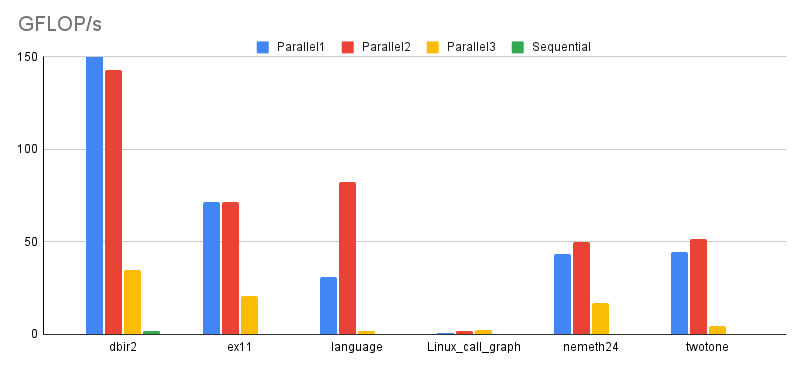
\includegraphics[width=1\linewidth]{images/GFLOP_s.png}
    \caption{Performance offerences between the four algorithms}
    \label{fig:flops-graph}
\end{figure}

\section{Results and conclusion}
The results indicates that:
\begin{itemize}
    \item The best situation is when the not null elements in the matrix are concentrated on the diagonal.
    \item If the number of not null elements per row is almost uniform for each row in the matrix, the first and the second parallel algorithms give similar results. 
    \item The second parallel algorithm behaves better in different situations than the others implementations thanks to its load distribution system.
    \item The third parallel algorithm is more performant that the others only if the number of not null elements per row is very large and the dispersion of the matrix is high.
\end{itemize}
Also the block size affects the performances of the algorithms. In facts:
\begin{itemize}
    \item In the first implementation the block size does not affect much the performances because the static allocation of workload. 
    \item In the second implementation a lower block size may reduce the concurrency on the assignment system of the rows. 
    \item In the third implementation a block size that is much lower that the average number of not null elements per row is more convenient because reduces significantly the concurrency introducted when accumulating the result on the output vector. 
\end{itemize}
\bibliographystyle{IEEEtran}
\bibliography{references}

\end{document}

